\documentclass[a4paper,11pt]{article}
\input{/home/tof/Documents/Cozy/latex-include/preambule_lua.tex}
\newcommand{\showprof}{show them}  % comment this line if you don't want to see todo environment
\fancyhead[L]{Initiation à la programmation}
\newdate{madate}{10}{09}{2020}
%\fancyhead[R]{\displaydate{madate}} %\today
\fancyhead[R]{Seconde - SNT}
%\fancyhead[R]{Première - NSI}
%\fancyhead[R]{Terminale - NSI}
\fancyfoot[L]{~\\Christophe Viroulaud}
\AtEndDocument{\label{lastpage}}
\fancyfoot[C]{\textbf{Page \thepage/\pageref{lastpage}}}
\fancyfoot[R]{\includegraphics[width=2cm,align=t]{/home/tof/Documents/Cozy/latex-include/cc.png}}

\begin{document}
\begin{Form}
\section{Problématique}
\begin{center}
\begin{tabular}{cc}
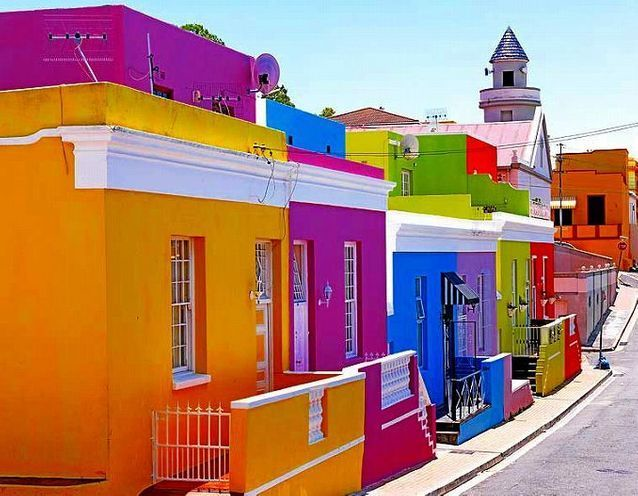
\includegraphics[width=3cm]{ressources/maisons-colorees.png}
 & 
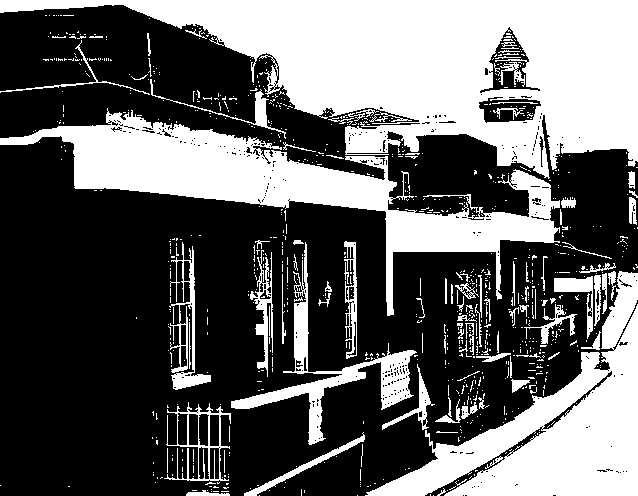
\includegraphics[width=3cm]{ressources/maisons-colorees-NB.png}
 \\ 
\end{tabular} 
\end{center}
Pour traiter une image automatiquement il faut utiliser un programme informatique: c'est une suite d'instructions destinées à être exécutée par une machine. Le \emph{Python} est un langage de programmation simple d'apprentissage.
\begin{center}
\shadowbox{\parbox{16cm}{\centering Quels éléments de programmation permettent de construire un programme informatique?}}
\end{center}
\section{Variable}
Pour stocker les informations dans un programme il faut les placer dans une variable.
\begin{center}
\begin{lstlisting}[language=Python]
a = 12
\end{lstlisting}
\captionof{code}{La variable \emph{a} contient la valeur 12.}
\label{moncode}
\end{center}
\begin{aretenir}[]
Le signe \textbf{=} affecte la valeur 12 à la variable \emph{a}.
\end{aretenir}
\begin{activite}
\begin{enumerate}
\item Créer un dossier \emph{photographie} dans l'espace personnel.
\item Ouvrir le logiciel \emph{Spyder} (dossier \emph{Maths} du bureau).
\item Dans la partie gauche, écrire le code \ref{variable}
\begin{center}
\begin{lstlisting}[language=Python]
a = 12
b = 8
c = a + b
print(c) # affiche le contenu de la variable c
\end{lstlisting}
\captionof{code}{Définir des variables}
\label{variable}
\end{center}
\item Enregistrer le programme dans le dossier \emph{photographie} sous le nom \emph{variable.py}
\item Exécuter le programme en cliquant sur la flèche verte (figure \ref{execution}) ou en appuyant sur la touche \emph{F5}. Le code est exécuté dans la console en bas à droite.
\begin{center}
\centering

\includegraphics[width=1cm]{ressources/execution.png}
\captionof{figure}{Exécuter un programme.}
\label{execution}
\end{center}
\end{enumerate}
\end{activite}
\section{Structure conditionnelle}
Il est souvent nécessaire de comparer le contenu de deux variables pour choisir le code à exécuter.
\begin{center}
\begin{lstlisting}[language=Python]
age = 15
if age < 18:
    print("Vous êtes mineur.")
else:
    print("Vous êtes majeur.")
\end{lstlisting}
\captionof{code}{Le texte affiché dépend de la variable \emph{age}.}
\label{majorite}
\end{center}
\begin{aretenir}[]
Le décalage (\emph{indentation}) des lignes 3 et 5 est indispensable. On le réalise avec \textbf{4 espaces} ou la touche de \emph{tabulation}.
\end{aretenir}
\begin{activite}
\begin{enumerate}
\item Dans un nouveau programme, écrire le code \ref{temp}
\begin{center}
\begin{lstlisting}[language=Python]
temperature = 10
if temperature == 0:
    print("L'eau commence à geler")
\end{lstlisting}
\captionof{code}{Pour vérifier l'égalité on utilise \textbf{==}}
\label{temp}
\end{center}
\item Modifier le code pour que le message s'affiche.
\end{enumerate}
\end{activite}
\section{Boucle}
Pour répéter une instruction on peut utiliser une boucle.
\begin{center}
\begin{lstlisting}[language=Python]
for compteur in range(10):
    print(compteur)
print("BOUM")
\end{lstlisting}
\captionof{code}{La boucle affiche la valeur de \emph{compteur} à chaque itération.}
\label{moncode}
\end{center}
\begin{activite}
Écrire un programme qui affiche les carrés des nombres de 0 à 10.
\end{activite}
\end{Form}
\end{document}